\documentclass[12pt]{article} 
\usepackage[utf8x]{inputenc}
\usepackage{graphicx} 
\usepackage{multirow} 
\usepackage{hhline}
\usepackage{booktabs} 
\usepackage{vmargin} %cambia el margen
\usepackage{amsmath,amsthm} 
\usepackage{amsfonts} 
\usepackage{float}
\usepackage{listings}
\usepackage{xcolor}

\usepackage{hyperref}

\hypersetup{
    bookmarks=true,         % show bookmarks bar?
    unicode=false,          % non-Latin characters in Acrobat’s bookmarks
    pdftoolbar=true,        % show Acrobat’s toolbar?
    pdfmenubar=true,        % show Acrobat’s menu?
    pdffitwindow=false,     % window fit to page when opened
    pdfstartview={FitH},    % fits the width of the page to the window
    pdftitle={Trabajo de mecánica celeste},    % title
    pdfauthor={Francisco Luque},     % author
    pdfsubject={Subject},   % subject of the document
    pdfcreator={Creator},   % creator of the document
    pdfproducer={Producer}, % producer of the document
    pdfkeywords={keyword1, key2, key3}, % list of keywords
    pdfnewwindow=true,      % links in new PDF window
    colorlinks=true,        % false: boxed links; true: colored links
    linkcolor=gray,         % color of internal links (change box color with linkbordercolor)
    citecolor=green,        % color of links to bibliography
    filecolor=magenta,      % color of file links
    urlcolor=blue           % color of external links
}

\title{
  Mecánica Celeste\\
  \large Trabajo de programación sobre la 
  órbita de los planetas en el sistema solar.  }


\author{ 
  Francisco Luque Sánchez
}

\begin{document}
\maketitle
\begin{center}  

\includegraphics[scale=0.35]{escudo.png}
\end{center}

\newpage

\tableofcontents % para generar el índice de contenidos

\pagebreak

\section{Introducción}

En esta práctica desarrollaremos un programa en Python que nos
permitirá conocer información sobre el estado de un planeta, visto
como una partícula en órbita en el Sistema Solar. Podremos calcular la
posición del mismo dependiendo del día del periodo orbital en el que
nos encontremos, así como su distancia al sol, la velocidad que tiene,
el módulo de la misma, su energía, su anomalía real y excéntrica, y su
momento angular.\\

Además, se nos permitirá representar en unos ejes cartesianos, en los
que se toma como punto de referencia el Sol, la órbita de los
planetas, así como su posición dentro de la órbita en un día
especificado por el usuario.\\

A lo largo de este informe vamos a explicar la fundamentación
matemática que justifica las funciones programadas en Python. El
código implementado se adjunta para su revisión en caso necesario.\\

Vamos ahora a ver la fundamentación matemática de las funciones
implementadas.

\section{Cálculos realizados}

Vamos a ver los cálculos realizados, que luego se han implementado
en funciones en Python para el programa.

\subsection{Posición de planeta}

Lo primero que se ha calculado es la posición del planeta. Para
calcular dicha posición, se ha utilizado el siguiente sistema:

\begin{equation}
  \left\{
    \begin{array}{l}
      x(t) = a(\cos{u(t)} - \varepsilon, \sqrt{1 - \varepsilon^2}\sin{u(t)}) \\
      u(t) - \varepsilon \sin{u(t)} = \frac{2\pi}{p}(t - t_0)      
    \end{array}
  \right.
  \label{eq:sist1}
\end{equation}

Lo primero que tenemos que calcular es la anomalía excéntrica. Hemos
supuesto $t_0 = 0$, ya que no tenemos información sobre un posible
punto de tiempo de referencia. Para poder calcular su valor, dado que
no podemos obtener una expresión analítica de la misma, vamos a
utilizar el método de Newton-Raphson para dar una aproximación
numérica.  Como ya vimos en las clases de teoría, definiendo
$\xi = \frac{2\pi}{p}$, y utilizando la expresión

\[
u_{n+1} = \frac{(-u_n\cos{u_n} + \sin{u_n})\varepsilon - \xi}{1 -
  \varepsilon \cos{u_n}}
\]

Tenemos una expresión iterativa basada en el método de Newton-Raphson
que nos permite aproximar el valor de la excentricidad en un tiempo
$t$.\\

Una vez calculado el valor de la anomalía excéntrica, simplemente 
sustituimos el valor en la ecuación de la posición, y obtenemos el
valor deseado.

\subsection{Distancia al Sol}

Para calcular la distancia al Sol, simplemente tendremos que calcular
el módulo de la posición calculada anteriormente.

\subsection{Velocidad del planeta}

Para calcular la velocidad, utilizaremos la derivada de la posición,
expresada de la misma manera que en apartado anterior. Tenemos que
dicha derivada es:

\[
\dot{x}(t) = a \dot{u}(t)(-\sin{u(t)}, \sqrt{1 -
  \varepsilon^2}\cos{u(t)})
\]

Y calculamos en clase que el valor de $\dot{u}(t)$ es:

\[
\dot{u}(t) = \frac{|c|}{a^2 \sqrt{1 - \varepsilon^2}(1 - \varepsilon
  \cos{u(t)})}
\]

Usando además la relación que nos liga el módulo del momento angular
con la longitud del semieje mayor de la elipse que define la órbita
del planeta, que es:

\[
a = \frac{|c|^2}{\mu(1 - \varepsilon^2)} \Rightarrow |c| =
\sqrt{a\mu(1 - \varepsilon^2)}
\]

Obtenemos que:

\[
\dot{u}(t) = \frac{\sqrt{a\mu}\sqrt{(1 - \varepsilon^2)}}{a^2 \sqrt{1
    - \varepsilon^2}(1 - \varepsilon \cos{u(t)})} =
\frac{\sqrt{a\mu}}{a^2 (1 - \varepsilon \cos{u(t)})}
\]

Ahora, con la tercera ley de Kepler podemos expresar $\mu$ en función
de otras constantes dependientes del planeta:

\[
p = \frac{2\pi}{\sqrt{\mu}}a^{\frac{3}{2}} \Rightarrow \sqrt{\mu} =
\frac{2\pi}{p}a^{3/2}
\]

Que sustituyendo en la ecuación, nos da el siguiente resultado:

\[
\dot{u}(t) = \frac{\sqrt{a\mu}}{a^2 (1 - \varepsilon \cos{u(t)})} =
\frac{2 \pi a^2}{a^2 p (1 - \varepsilon \cos{u(t)})} = \frac{2 \pi} {p
  (1 - \varepsilon \cos{u(t)})}
\]

Ahora sustituimos este valor en la expresión de $\dot{x}(t)$ para
obtener una expresión de la velocidad dependiente del tiempo:

\[
\dot{x}(t) = \frac{2 \pi a}{p(1 - \varepsilon
  \cos{u(t)})}(-\sin{u(t)}, \sqrt{1 - \varepsilon^2}\cos{u(t)})
\]

De nuevo, el cálculo de la anomalía excéntrica se hace con el método
de Newton-Raphson anteriormente explicado.

\subsection{Módulo de la velocidad}

Para obtener el módulo de la velocidad, calculamos la norma del
vector anterior.

\subsection{Anomalía real}

Además del sistema de ecuaciones anterior, la posición de un planeta
se puede expresar también con el siguiente sistema de ecuaciones:

\begin{equation}
  \left\{
    \begin{array}{l}
      x(t) = \frac{a(1 - \varepsilon^2)}{1 + \varepsilon(\cos{\theta(t)} - \omega)}(\cos{\theta(t)}, \sin{\theta(t)})\\
      \dot{\theta}(t) = \frac{|c|}{a^2(1 - \varepsilon^2)^2}(1 + \varepsilon \cos{(\theta(t) - \omega)})
    \end{array}
  \right.
  \label{eq:sist2}
\end{equation}

La función $\theta(t)$ se conoce como la anomalía real del planeta, y
marca el ángulo que forma, en radianes, el planeta con el semieje
mayor positivo de la elipse. Queremos averiguar dicho valor para un
tiempo $t$, pero no podemos obtener una expresión analítica de dicha
función, por lo que para resolverlo utilizaremos el método de
Runge-Kutta-4. Este método numérico sirve para estimar valores de una
función en un determinado punto $t$, conocida una expresión de la
derivada de la función a estimar (en nuestro caso una expresión de
$\dot{\theta}(t)$, que tenemos escrita en el sistema anterior), y una
pareja $(t_0, \theta(t_0))$. Interpretando el significado de la
fúnción $\theta$, y suponiendo que $\omega = 0$, que indica el giro
del semieje mayor de la elipse respecto del eje $OX^{+}$, tenemos que
$\theta(t_0) = 0$, que será el punto de referencia que tomaremos
para utilizar el método seleccionado.\\

No haremos una explicación más profunda del funcionamiento de dicho
método, ya que se sale de los contenidos de la asignatura. Se puede
ver una explicación del método en
\url{https://en.wikipedia.org/wiki/Runge%E2%80%93Kutta_methods}

\subsection{Energía del planeta}

Pasamos ahora al cálculo de la energía del planeta. Por un lado,
tenemos que la energía de un cuerpo sometido a un campo de fuerzas
centrales en un determinado instante de tiempo $t$ es la siguiente:

\[
E_{t}(t) = E_{c}(t) + E_{p}(t) = \frac{m|\dot{x}(t)|^2}{2} -
\frac{m\mu}{|x(t)|}
\]

Donde nos aparecen involucrados el módulo de la velocidad del planeta,
anteriormente calculado, la distancia al Sol del mismo, cálculo que
también hemos realizado, y la constante $\mu$, para la que vimos antes
la expresión:

\[
\sqrt{\mu} = \frac{2\pi}{p}a^{3/2} \Rightarrow \mu = \frac{4
  \pi^2}{p^2}a^3
\]

Por lo que podemos calcular de forma sencilla el valor de la energía
en un determinado instante de tiempo $t$. Además, se dedujo, con la
ley de conservación de la energía, que la energía en todo momento es
constante. Podemos calcular entonces una expresión de la energía en
función de las constantes del planeta, que nos permita calcularla sin
tener que recurrir a la evaluación de la distancia al Sol y el módulo
de la velocidad en un instante de tiempo determinado. No mostramos
todos los cálculos intermedios dado que es un proceso tedioso, pero la
expresión de la energía la podemos calcular de la siguiente
manera. Tenemos por un lado que la distancia del planeta al Sol es,
tomando como posición el primer sistema que mostramos en la práctica:

\[
|x(t)| = a(1 - \varepsilon \cos{u(t)})
\]

Por otro, el cuadrado del módulo de la velocidad se puede expresar
como:

\[
|\dot{x}(t)|^2 = a^2|\dot{u}(t)|^2(1-\varepsilon^2cos^2{u(t)})
\]

Sustituyendo dichos valores en la expresión que pusimos al principio,
obtenemos:

\[
E_{t}(t) = \frac{ma^2|\dot{u}(t)|^2(1-\varepsilon^2cos^2{u(t)})}{2} -
\frac{m\mu}{a(1 - \varepsilon \cos{u(t)})}
\]

El valor del módulo de $|\dot{u}(t)|^2$ sabemos que es:

\[
|\dot{u}(t)|^2 = \frac{|c|^2}{a^4(1-\varepsilon^2)(1 - \varepsilon
  \cos{u(t)})^2}
\]

Y conocemos la siguiente expresión para $\mu$:

\[
\mu = \frac{|c|^2}{a(1 - \varepsilon^2)}
\]

Al sustituir ambos valores en la expresión anterior y simplificar, se
obtiene que:

\[
E_t(t) = \frac{m|c|^2(1+\varepsilon
  \cos{u(t)}}{2a^2(1-\varepsilon^2)(1-\varepsilon \cos{u(t)})} -
\frac{m|c|^2}{a^2(1 - \varepsilon^2)(1-\varepsilon \cos{u(t)})}
\]

Convirtiendo las dos fracciones a común denominador, llegamos a la
siguiente expresión:

\[
E_t(t) = -\frac{m|c|^2}{2a^2(1-\varepsilon^2)}
\]

Que claramente es independiente del tiempo. El único valor que
tendríamos que calcular es el módulo del momento angular, que veremos
en la siguiente sección que es también constante. De esta forma,
tenemos una expresión constante para la energía, que en la
implementación compararemos con la energía en un instante de
tiempo, para comprobar la corrección de los cálculos.\\

Dado que no tenemos datos sobre la masa de los planetas, la
implementación de la energía que daremos será por unidad de masa. Para 
obtener el dato de la energía real de un planeta, habría que multiplicar
el valor que obtengamos por la masa del mismo.

\subsection{Momento angular del planeta}

De nuevo el cálculo del momento angular puede ser realizado de dos
formas distintas. Tenemos, por un lado, una expresión dependiente del
tiempo, y por otro, por la ley de conservación del momento sabemos que
podemos encontrar una expresión constante para el mismo, dependiente
de las constantes propias del planeta. Comenzamos viendo la expresión
dependiente del tiempo. En clase calculamos una expresión del mismo,
que es la siguiente:

\[
c(t) = r(t)^2\dot{\theta}(t)(0,0,1)
\]

Dado que estamos trabajando suponiendo que todos los planetas están en
el plano $XY$, y el momento angular es perpendicular al plano en el
que se mueve el planeta, las dos primeras componentes del momento
angular son nulas. Es por esto que en lugar de trabajar con el momento
angular como un vector, trabajaremos con el módulo del momento
escalar, que coincide con el valor de su tercera componente. Por
tanto, la expresión que daremos del mismo es

\[
|c(t)| = r(t)^2\dot{\theta}(t)
\]

Donde $r(t)$ es la distancia al Sol del planeta, y $\dot{\theta}(t)$
la podemos obtener de \ref{eq:sist2}. Vamos ahora a ver la expresión
constante del módulo del producto escalar. Teniendo en cuenta que el
planeta se mueve en una elipse, llegamos a la relación:

\[
a = \frac{|c|^2}{\mu(1 - \varepsilon^2)} \Rightarrow |c| =
\sqrt{a\mu(1 - \varepsilon^2)}
\]

Mostraremos ambos valores en el programa, para comprobar empíricamente
que el módulo del momento angular calculado con la expresión
dependiente del tiempo coincide con el valor constante,
independientemente del momento de tiempo en el que hagamos el cálculo.

\subsection{Anomalía real en función de la anomalía excéntrica}

Vamos ahora a mostrar otra forma de calcular la anomalía real para un
planeta en un instante de tiempo $t$. Ya hemos visto que podemos
aproximar el valor de la anomalía real utilizando el método de
Runge-Kutta, dado que tenemos una expresión de $\dot{\theta}(t)$ y
sabemos que $\theta(0) = 0$. Otra forma que tenemos de realizar este
cálculo es, sabiendo que tanto la anomalía excéntrica como la real son
funciones biyectivas de $[0, p)$ en $[0, 2\pi)$, donde $p$ es el
periodo de rotación del planeta, tratar de expresar $\theta$ en
función de $u$. Como tenemos ambas funciones son biyectivas en los
intervalos que hemos dicho, podemos establecer una biyección entre
ambos valores.  Para ello, utilizaremos como paso intermedio la
expresión de la posición de un planeta en un instante de tiempo
$t$. Pasamos a ver dicha expresión.  Tomando la primera componente de
la posición expresada en el sistema \ref{eq:sist2}, tenemos que:

\[
x(t) = \frac{a(1 - \varepsilon^2)\cos{\theta(t)}}{1 +
  \varepsilon\cos{\theta(t)}} \Rightarrow \cos{\theta(t)} =
\frac{x(t)(1 + \varepsilon\cos{\theta(t)})}{a(1 - \varepsilon^2)}
\Rightarrow
\]
\[
\Rightarrow \cos{\theta(t)} = \frac{x(t) + \varepsilon x(t)
  \cos{\theta(t)}} {a(1 - \varepsilon^2)} \Rightarrow \cos{\theta(t)}
- \frac{\varepsilon x(t) \cos{\theta(t)}} {a(1 - \varepsilon^2)} =
\frac{x(t)}{a(1 - \varepsilon^2)} \Rightarrow
\]
\[
\Rightarrow \cos{\theta(t)}\left(\frac{a(1 - \varepsilon^2) -
    \varepsilon x(t)}{a(1 - \varepsilon^2)}\right) = \frac{x(t)}{a(1 -
  \varepsilon^2)} \Rightarrow \cos{\theta(t)} = \frac{x(t)}{a(1 -
  \varepsilon^2) - \varepsilon x(t)} \Rightarrow
\]
\[
\Rightarrow \cos{\theta(t)} = \frac{\frac{x(t)}{a}}{1 - \varepsilon^2
  - \varepsilon \frac{x(t)}{a}}
\]

Ahora, tomando la primera componente de la posición en el sistema
\ref{eq:sist1}, tenemos que

\[
\frac{x(t)}{a} = \cos{u(t)} - \varepsilon
\]

Que sustituyendo en la igualdad anterior nos deja

\[
\cos{\theta(t)} = \frac{\cos{u(t)} - \varepsilon}{1 - \varepsilon^2 -
  \varepsilon(\cos{u(t)} - \varepsilon)} = \frac{\cos{u(t)} -
  \varepsilon}{1 - \varepsilon\cos{u(t)}}
\]

Finalmente, aplicando la función arco coseno, tenemos que

\[
\theta(t) = \arccos\left(\frac{\cos{u(t)} - \varepsilon}{1 -
    \varepsilon\cos{u(t)}}\right)
\]

Por tanto, hemos conseguido expresar la anomalía real en función
de la anomalía excéntrica, por lo que podemos calcular un valor
en función del otro. En el programa, lo que tendremos será una
función que nos acepte un tiempo $t$, respecto de ese tiempo se
calcula el valor de la anomalía excéntrica, y con ese valor de
anomalía excéntrica se calcula el valor de la anomalía real usando
la relación anterior.

\subsection{Anomalía excéntrica con funciones de Bessel}

El último apartado de la práctica consiste en calcular el valor de la
anomalía excéntrica utilizando para ello funciones de Bessel. Vimos
en clase la siguiente expresión:

\[
u(t) = \frac{2 \pi (t - t_0)}{p} + \sum \frac{2}{n} J_n(n\varepsilon)
\sin{\frac{2 \pi n(t - t_0)}{p}}
\]

Donde $J_n$ es la función de Bessel de orden $n$. Suponiendo como
hemos hecho en el resto de la práctica que $t_0 = 0$, daremos esta
implementación en el programa, de forma que para un determinado $t$ se
imprima el valor de la anomalía excéntrica calculado por el método
de Newton-Raphson y a partir de las funciones de Bessel, y comprobaremos
que llegamos a resultados similares.

\section{Aspectos de implementación y ejecución de la práctica}

Vamos ahora a comentar ciertos aspectos de la implementación que se ha
realizado. Todo el código se ha implementado en Python 3. Dicho código
se encuentra adjunto en el archivo comprimido de la práctica, y
también
está disponible en \url{https://github.com/pacron/celeste}.\\

Para crear un entorno interactivo y sencillo de utilizar para el
usuario se ha utilizado la herramienta Jupyter
(\url{http://jupyter.org/}). Esta herramienta permite crear entornos
interactivos de Python, de forma que es sencillo compartir el código
desarrollado para que otros usuarios lo
ejecuten, sin necesidad de que instalen Python en su ordenador.\\

Además, para simplificar aún más la forma de compartir la información
a otros usuarios y que puedan ejecutar el código desarrollado, se ha
creado un entorno virtual para ejecutarlo, haciendo uso de la
plataforma \textit{mybinder}.  Concretamente, copiando el enlace
\url{https://mybinder.org/v2/gh/pacron/celeste/master?filepath=celeste.ipynb}
en un navegador se accede al entorno interactivo. Lo único que hay que
hacer es esperar a que el sistema cargue los archivos y se redigirá 
a una ventana en la que se puede interactuar con el código. La ventana
en cuestión es la siguiente:

\begin{figure}[H]
  \centering
  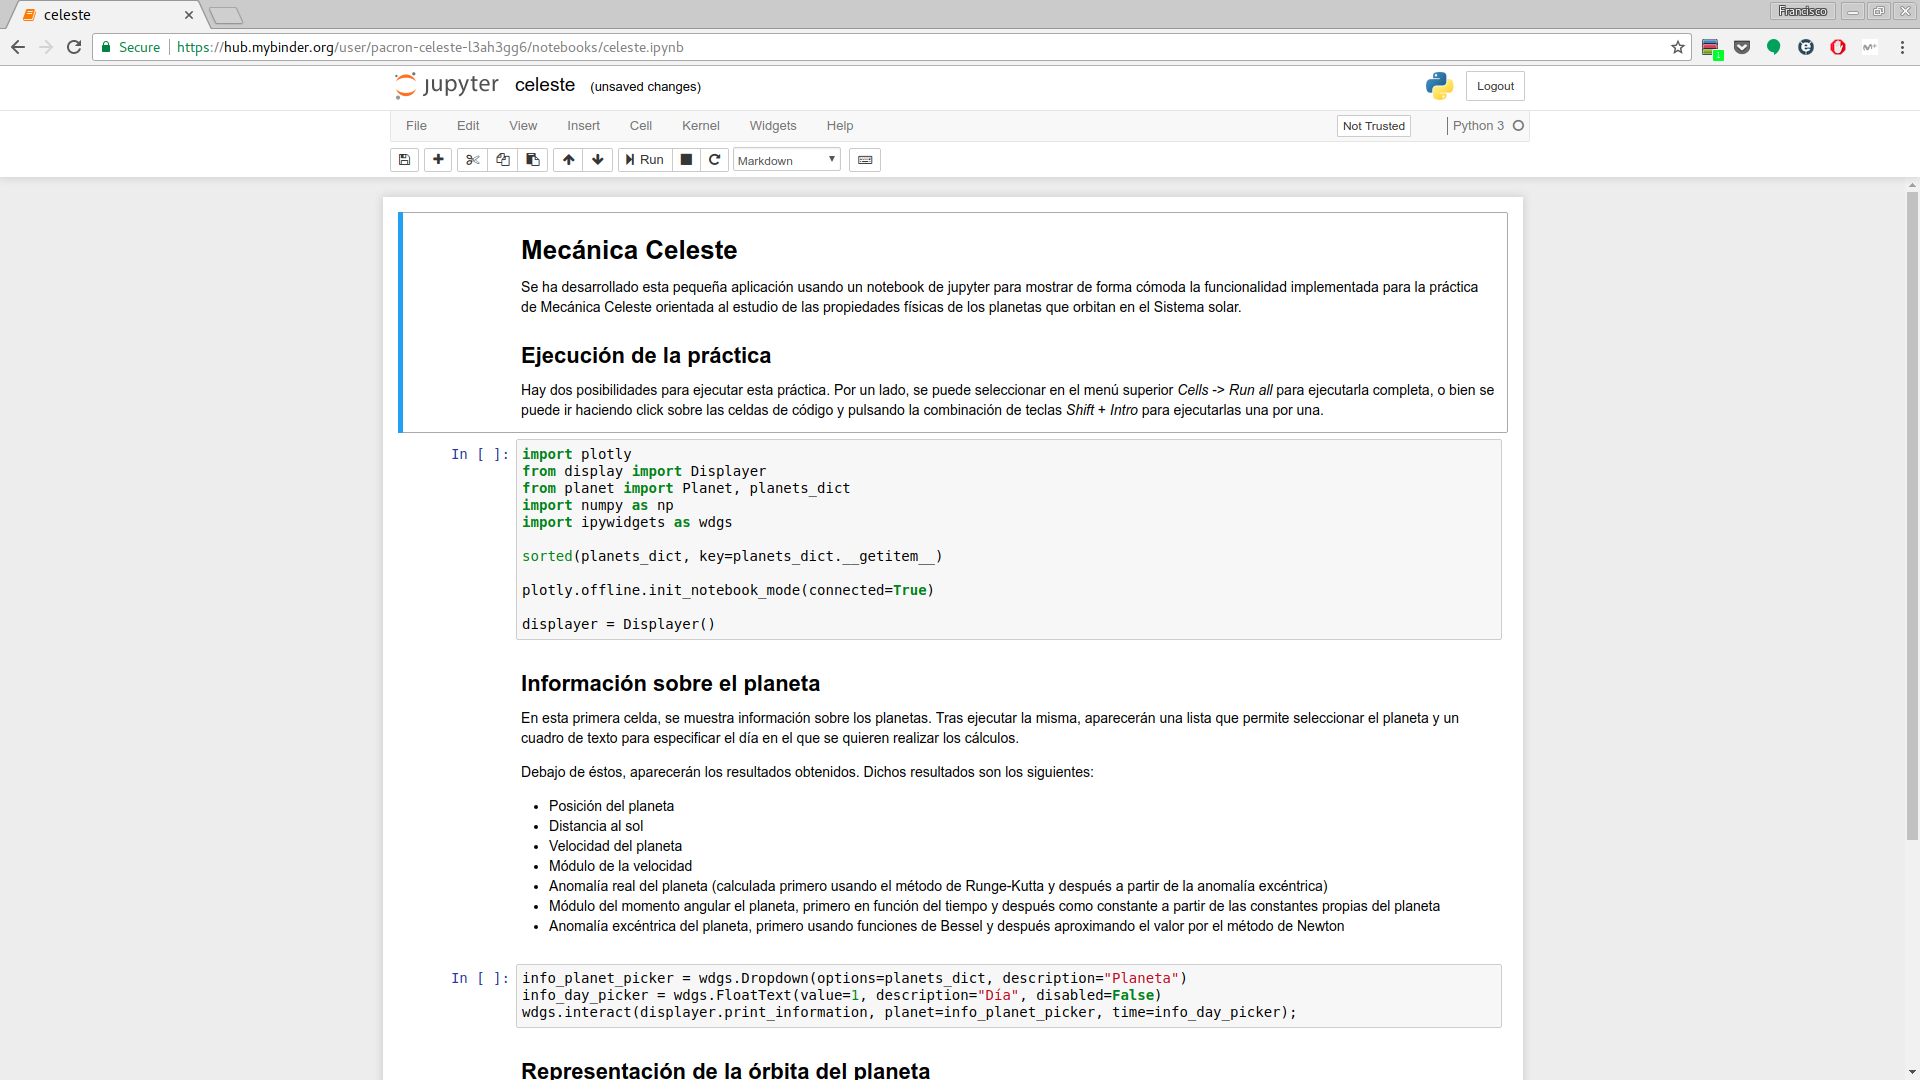
\includegraphics[width=.9\textwidth]{imgs/notebook}
  \caption{Ventana de ejecución de Jupyter}
\end{figure}

Ahora, haciendo click en \textit{Cell $\rightarrow$ Run all} tal y como
se muestra en la siguiente imagen, se ejecutan todas las celdas de código
y se muestran los resultados de la práctica obtenidos:

\begin{figure}[H]
  \centering
  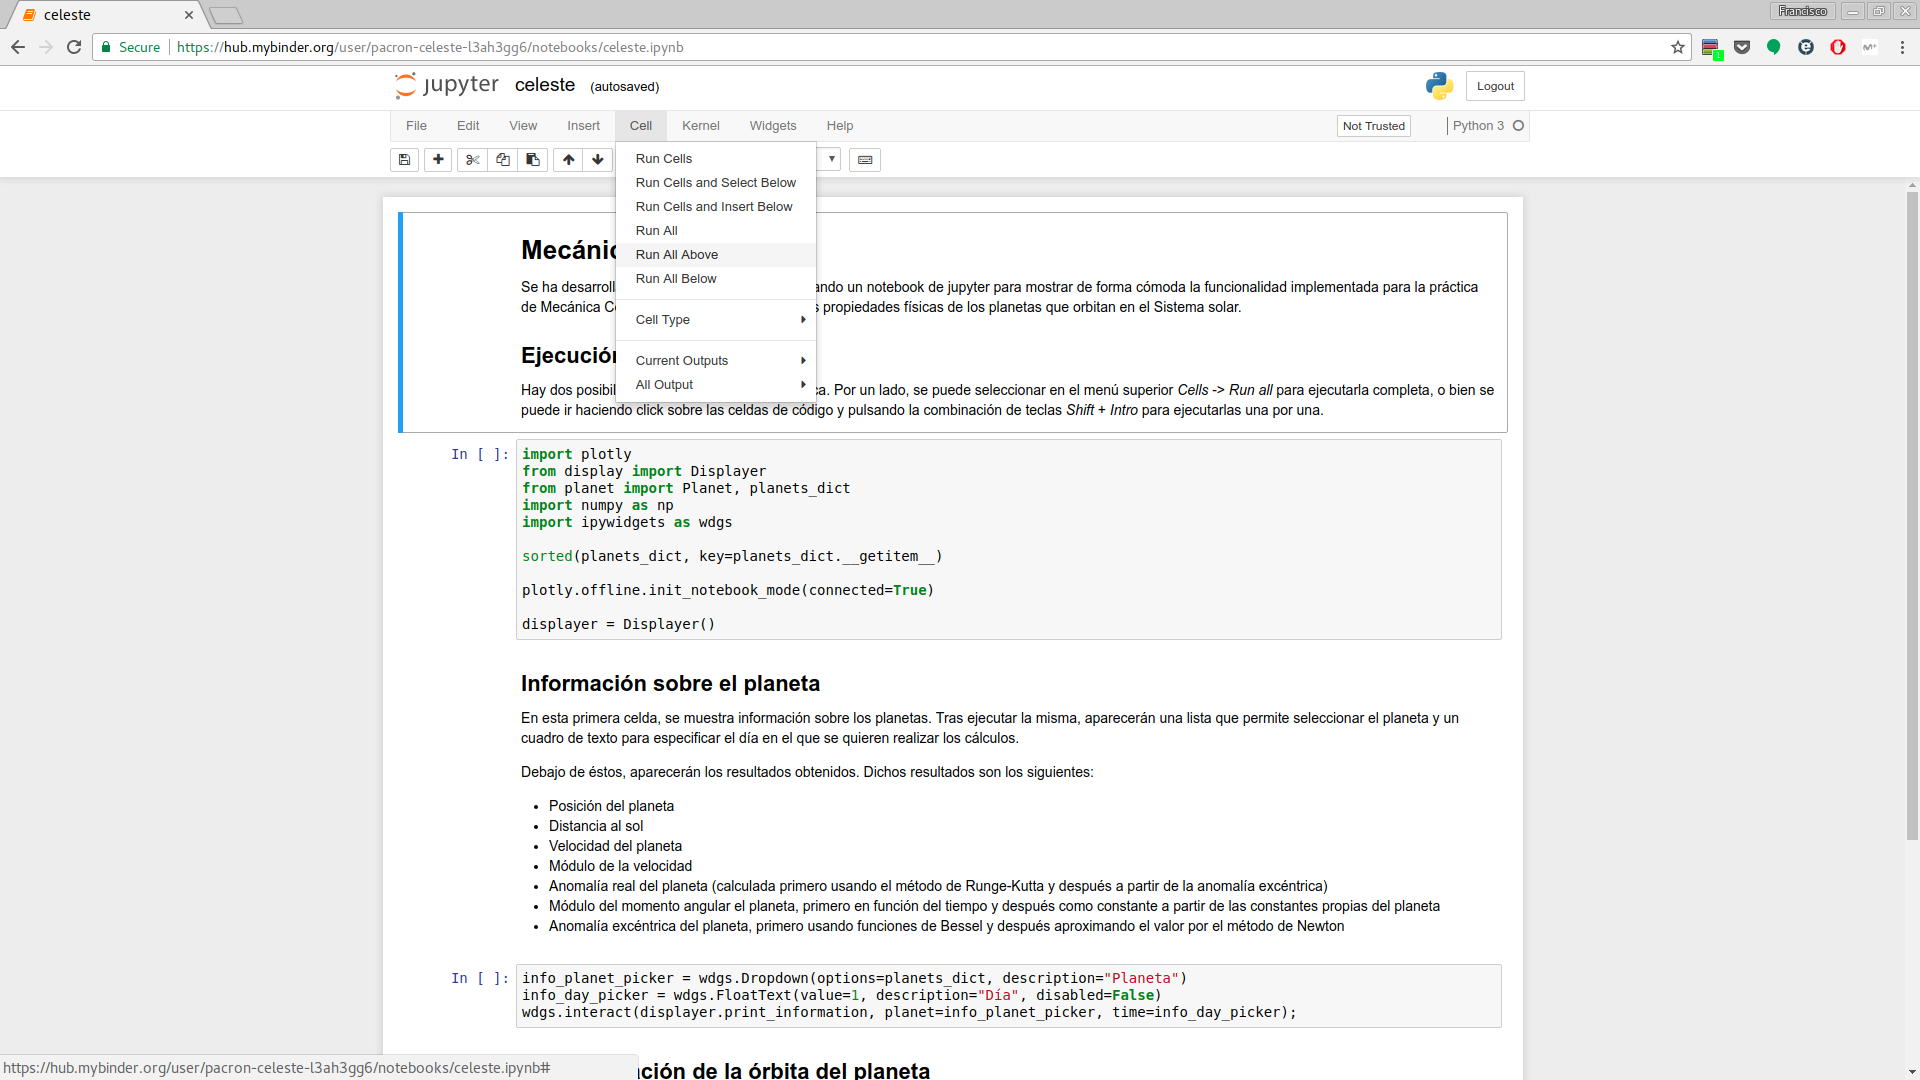
\includegraphics[width=.9\textwidth]{imgs/run_all}
  \caption{Ejecución de todas las celdas de código}
\end{figure}

Una vez realizada la ejecución, debajo de las dos celdas de código apareceran
dos objetos con los que se puede interactuar. Por un lado, un desplegable
que nos permite seleccionar el planeta sobre el que queremos obtener información,
y por otro, un cuadro de texto para seleccionar el día del periodo orbital en
el que se quiere obtener dicha información.\\

En la primera celda aparece la información sobre los parámetros calculados
para el planeta en cuestión el día seleccionado, tal y como se muestra en 
la figura siguiente. Para el ejemplo que se muestra se ha tomado la Tierra
en el día 100 del periodo:

\begin{figure}[H]
  \centering
  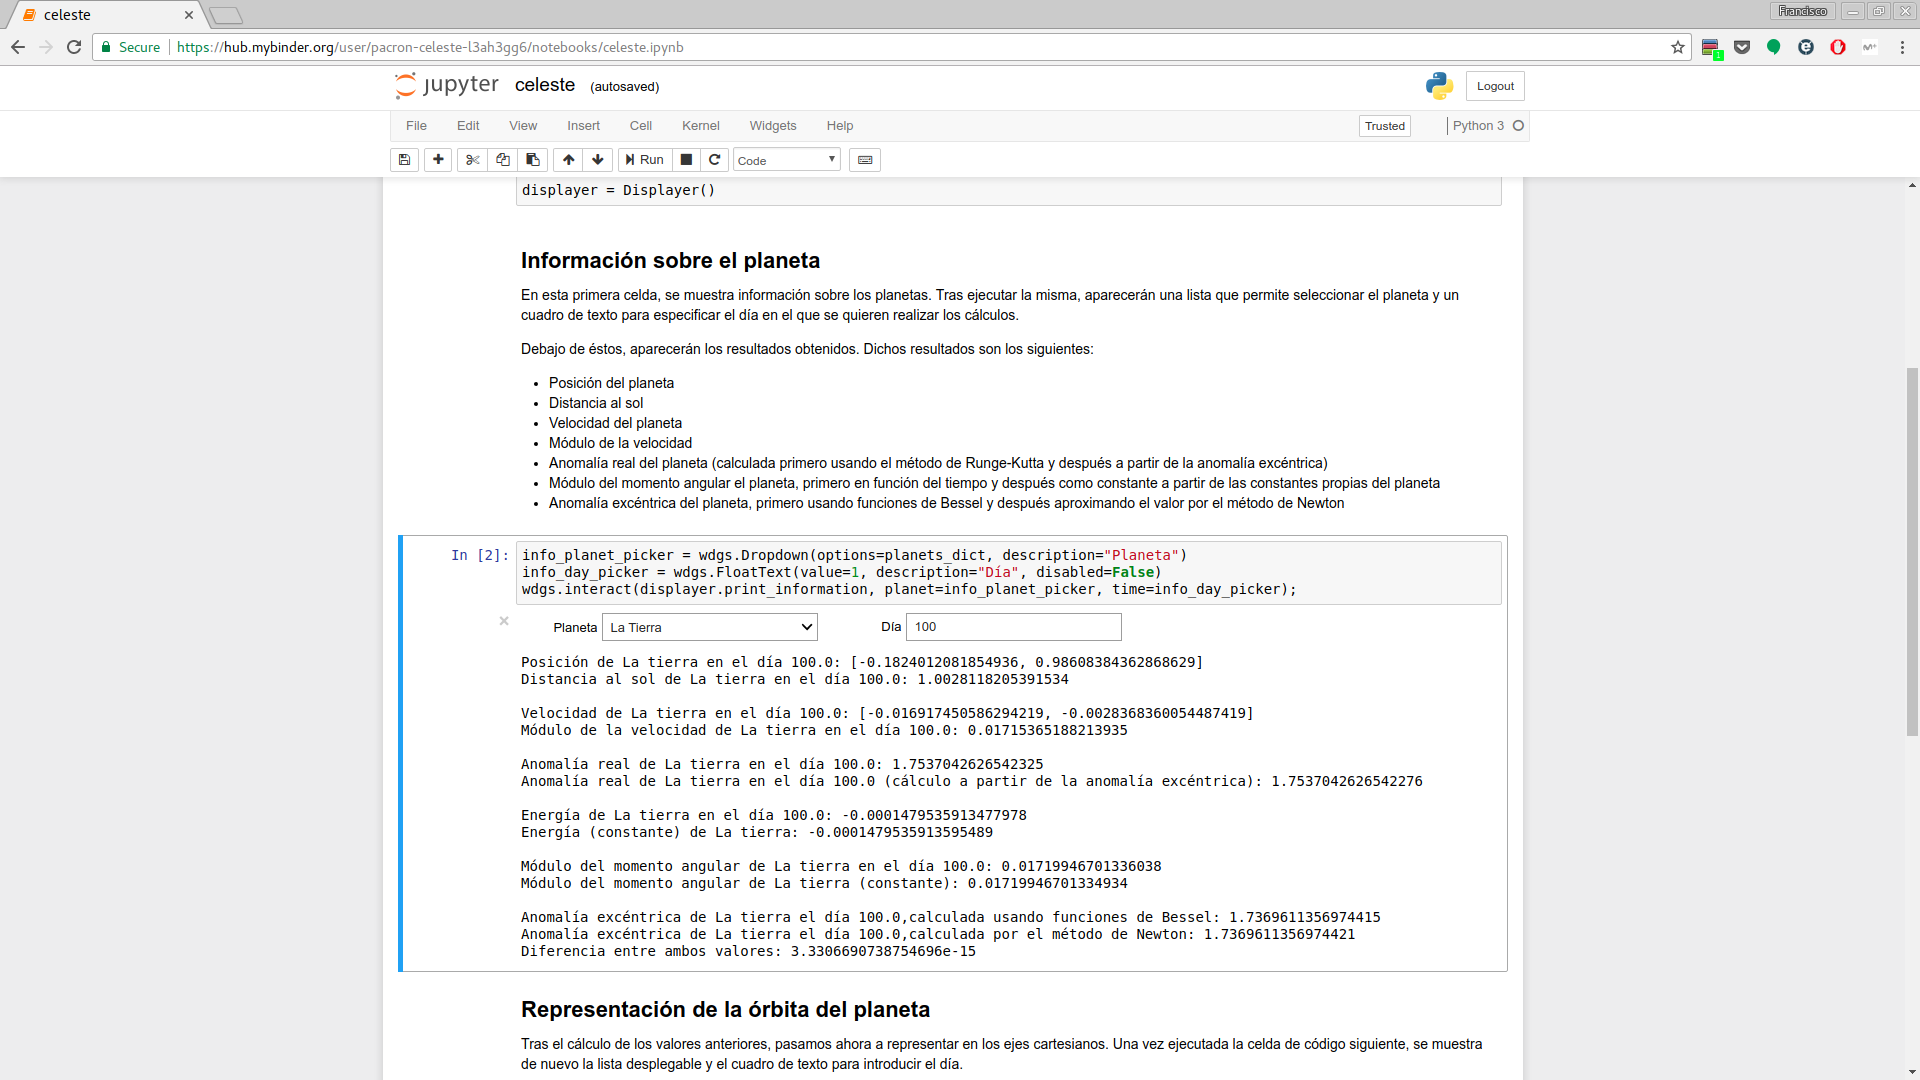
\includegraphics[width=.9\textwidth]{imgs/earth_information}
  \caption{Información calculada para la Tierra en el día 100 del periodo orbital}
\end{figure}

En la segunda celda, se muestra también para el planeta seleccionado, un
gráfico con la órbita del mismo. Se muestran tres objetos en la gráfica.
En el origen de coordenadas aparece el Sol, ya que es el punto que se
toma como referencia. En azul, se muestra la órbita elíptica alrededor
del Sol, y con un punto rojizo de mayor tamaño la posición que ocupa
el planeta en el día especificado. De nuevo, en el ejemplo que se
muestra a continuación aparece la Tierra en el día 100 del periodo
orbital:

\begin{figure}[H]
  \centering
  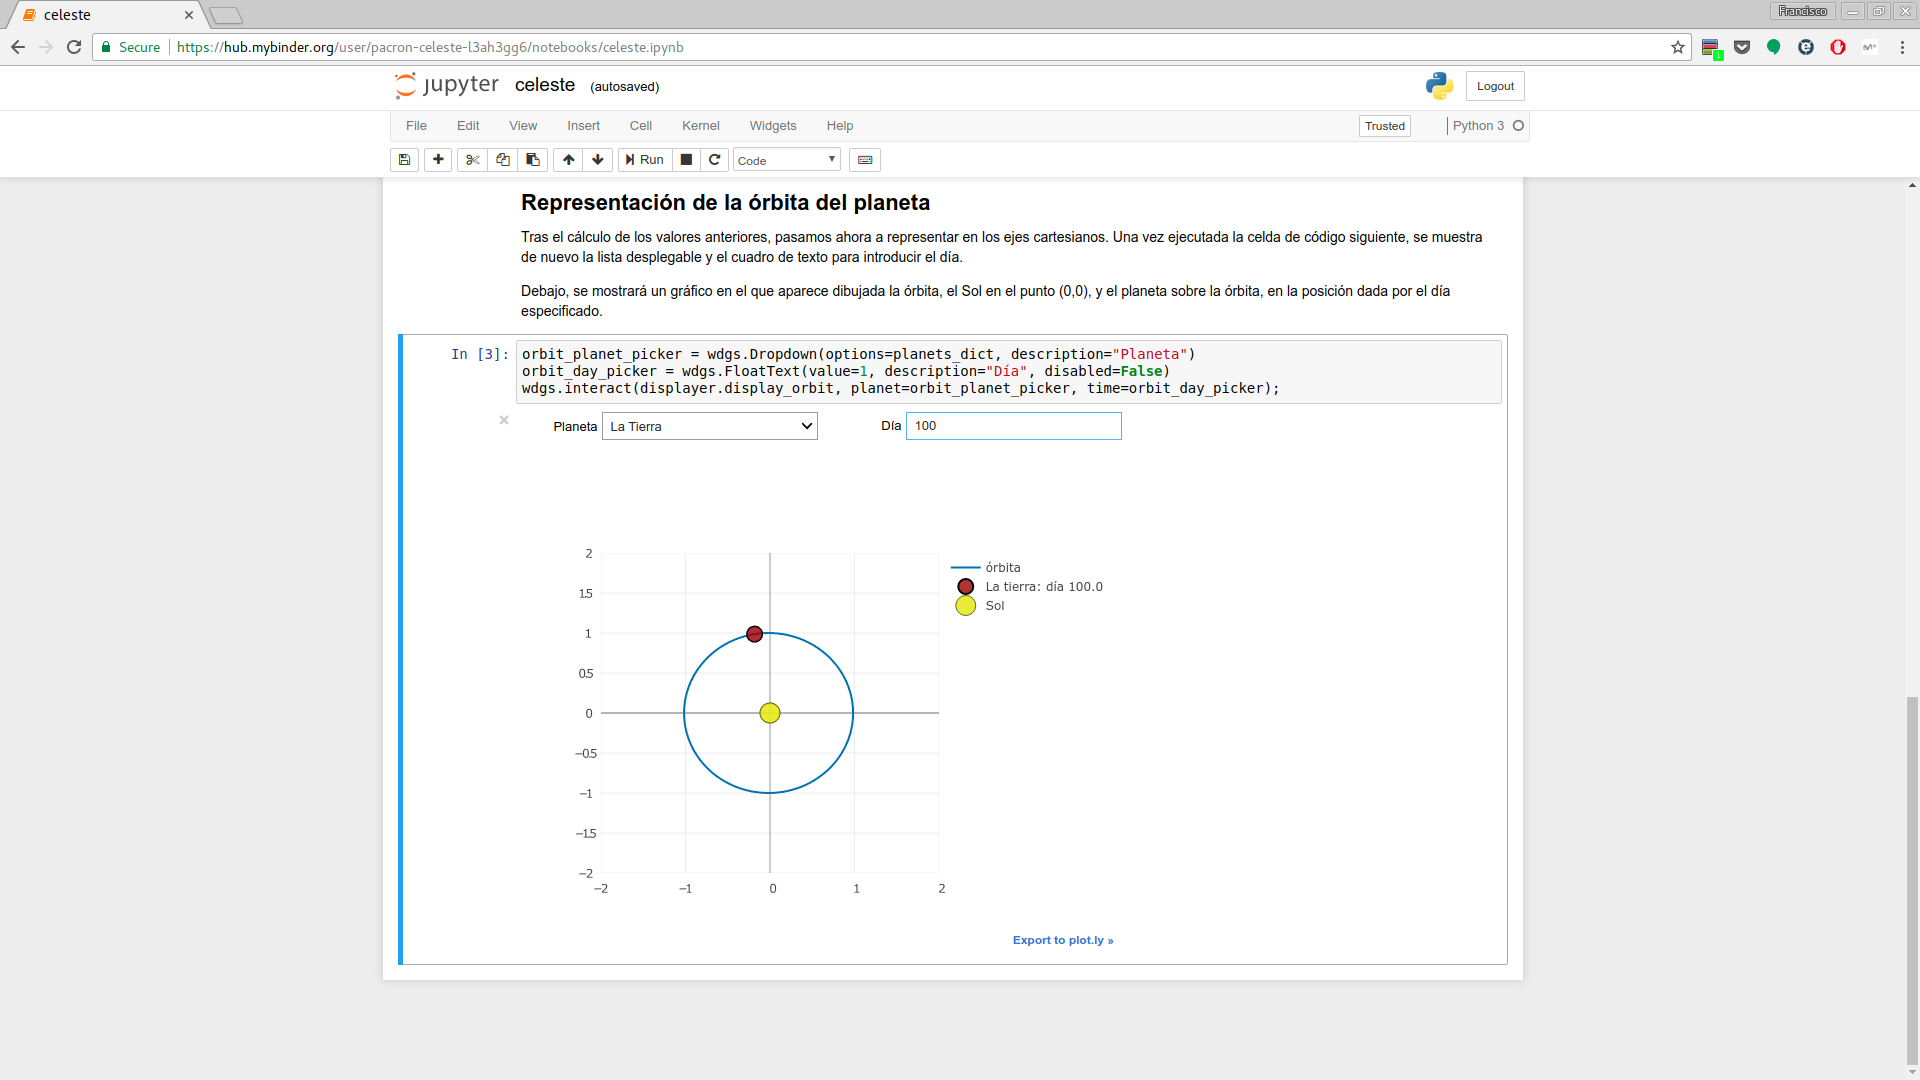
\includegraphics[width=.9\textwidth]{imgs/earth_orbit}
  \caption{Órbita de la Tierra alrededor del Sol (posición en el día 100)}
\end{figure}

\end{document}